Face detection and recognition is not a new subject to computer science. Through time there were many attempts to provide satisfactory solution and approximation. Techniques used for face detection spans from regular well known image recognition via edge detection, to more advanced, precise, though computationally expensive use of neural networks. This chapter will provide a basic overview of the mainstream approaches, listing the most current state-of-the-art methods and means to the problem.

Each section in this chapter represents a family of solutions. Providing a full description, explanation and understanding of their respective problem would span a book of its own, hence we aim to cover only a high level walk-though. We may also revisit certain aspects in more detail in later the text, as well.

\section{Convolutional neural networks}

There are many kinds of neural networks, one of which is called Convolutional Network\,\cite[p.~330]{deeplearningbook}, or CNN (Convolutional Neural Network). CNN specialises in processing data of known, grid-like structure. That includes for example time-series data, which can be represented as one dimensional grid of samples taken in regular time intervals. It also includes image data, represented as 2D grid of pixels. As the name suggests, CNNs employs a mathematical operation called \textbf{convolution}. In practical application, that stands for a substitution of a matrix multiplication by this linear mathematical operation - convolution. And this is done so in at least one of the network's layers.

This section aims to explain what convolution is, what are the motivations behind its usage in neural networks. Later we'll describe a \textbf{pooling} operation, which is used in almost all CNNs as well.

\subsection{Convolution}

Convolution as a mathematical operation generally symbolise an operation on two functions of real-valued argument. Let's start with an example of such functions and demonstrate a motivation behind convolution:

Assume we have a vehicle and a laser parking sensor mounted on its front. This sensor is used to measures a distance to some object, let's say a docking station for the vehicle. And we want to park the vehicle at some precise proximity to the object. The sensor provides an single output $p(t)$, which reads as a position of the vehicle at certain time. Both $p$ and $t$ are real-valued, which means that the sensor can provide a different output value at any instance in time.

We also have to count in that our sensor is not always fully precise and reliable, so the measurements provided may be noisy. To obtain a more relevant data we\,--\, less noisy estimate of the position against the object, we can base our measurement on an average of several data samples. Since the vehicle is moving, we have to assume that more recent outputs should provide more relevant reading. So, we can weight our average and give the more recent data points more importance. Let's define this weight function as $w(a)$, where the argument $a$ symbolize age of a measurement.

Calculating the weighted average at every moment, we can get a smoother estimation of the vehicle's position as a new function:

\begin{equation}
    s(t) = \int p(a) w(t - a) da
\end{equation}


The function $s$ is formally known as \textbf{convolution}. An asterisk symbol is usually used to denote this operation:

\begin{equation}
    s(t) = (p * w)(t)
\end{equation}

To complete the definition, we have to note that $w$ has to be a valid probability density function, which in our example has to meet a criteria $a < 0: w(a) = 0$. That limits our function to weight only past samples, since we can's assume that our sensor can look into the future, that would be silly. That is a limitation to our use case only. In general, convolution is defined for all functions where the integral above is defined.

Convolutional neural networks use a bit different terminology, than we used in the example. The function providing data we want to consume ($p$ from the example) is simply called \textbf{input}. The other parameter to the convolution, in our example that was the weight function, is called a \textbf{kernel}. The result of convolution ($s$) of input ($p$) over a kernel ($w$) is simply called \textbf{output} or \textbf{feature map}.

Our expectation that the sensor from example above would provide a measurement continuously, in any instant of time, is not realistic. Time is usually discretized in digital world, therefore it's meaningful to assume the sensor is providing measurements at regular intervals. Therefore instead od integrating over time continuum, we can define discrete convolution as:

\begin{equation}
    s(t) = \sum_{a=-\infty}^{\infty} p(a) w(t - a) = (p * w)(t)
\end{equation}

Our example was quite simple and straightforward, usually in artificial intelligence and deep-learning the input is common to be multidimensional array (tensor) of data. Also the kernel happens to be a tensor of parameters which values are often obtained by some learning algorithm.

Finally, when processing multidimensional data convolution is used over multiple axis at the same time. That's important for our application, because processing pictures have more than one dimension. So in case we have an input image $I$\,--\, a two-dimensional bitmap, our convolution should use a two-dimensional kernel $K$ as well:

\begin{equation}
    S(x,y) = (I * K)(x, y) = \sum_i\sum_j I(m, n) K(x - i)(y - j)
\end{equation}

\begin{figure}[ht]
    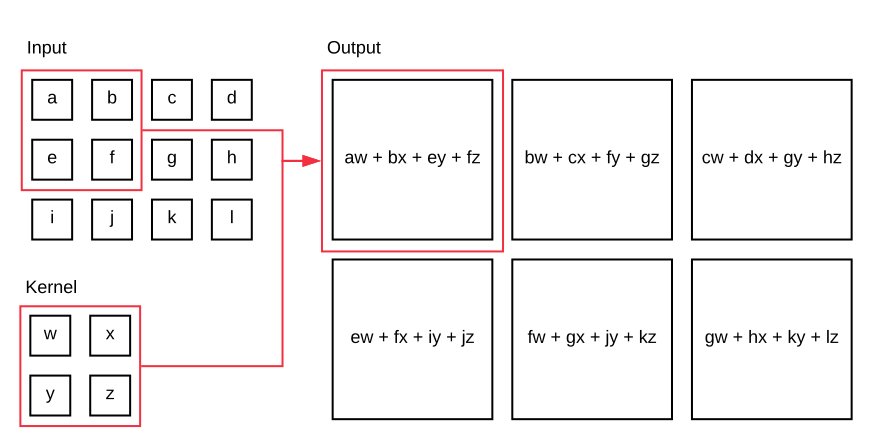
\includegraphics[width=\textwidth]{obrazky-figures/convolution.pdf}
    \caption{Convolution operation with 2D input data and 2D kernel}\label{fig:convolution}
\end{figure}

\subsection{Use of convolution in neural networks}

In machine learning, we leverage multiple important properties of the convolution operation:

\begin{itemize}
    \item Sparse interaction
    \item Sharing of parameters
    \item Equivariant representation
    \item Input of variable size
\end{itemize}

\subsubsection{Sparse interaction}

As you can notice in figure\,\ref{fig:convolution}, kernel can be of different size than input. When the input data is for example an image of millions of pixels, the size of kernel allows convolution to select only specific subset of inputs for each output. In traditional neural networks matrix multiplication is used instead of convolution. That means every output unit interacts with every input unit. In convolutional networks, the kernel size limits that just to certain subset of input units. It is called \textbf{sparse interaction}\,\cite[p.~335]{deeplearningbook} or \textbf{sparse weights} and it is accomplished by restricting kernel to a smaller size than the input. That results in smaller memory footprint of the model, since it requires fewer parameters to be stored. while at the same time it improves statistical efficiency. It has also impact on performance, since computing the output requires fewer operations compared to matrix multiplication. A graphical demonstration can be seen on figure\,\ref{fig:sparse_b}.

\begin{figure}[ht]
    \centering
    \includegraphics[width=.6\textwidth]{obrazky-figures/sparse_b.pdf}
    \caption{\textit{Sparse interaction viewed from below}: The highlighted units demonstrates propagation of one input unit from current layer $s_3$ to the next layer. On the top you can see all the output $n$ units, which are affected by this particular input. On the bottom image, you can see how the same situation is represented in traditional matrix multiplication.}\label{fig:sparse_b}
\end{figure}

Deep convolutional networks allow indirect interaction between units which would be out of reach for given kernel size. This property is called \textbf{receptive field}\,\cite[p.~337]{deeplearningbook} of a unit and can be seen when we look at the network from perspective of the output layer (see figure\,\ref{fig:sparse_a}).

\begin{figure}[ht]
    \centering
    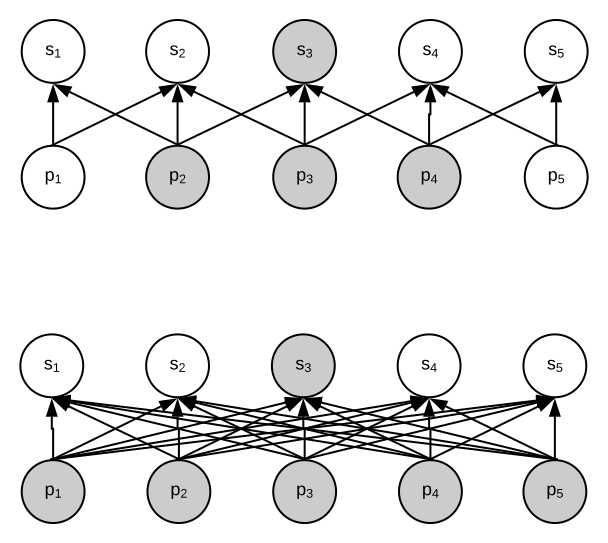
\includegraphics[width=.6\textwidth]{obrazky-figures/sparse_a.pdf}
    \caption{\textit{Sparse interaction viewed from above}: Highlighted portion of the image shows all units affecting current layer. The amount of units is smaller on the top picture. That represents sparse interaction. On the bottom is the same situation, when the current layer is formed by matrix multiplication in a traditional network.}\label{fig:sparse_a}
\end{figure}

However, this view limits us just to direct influence on a unit. Receptive field lists also indirect influence, hence when multiple convolutional layers are used by the network the field grows. The effect can be enhanced when network contains additional features like strided convolution or pooling. This means though the direct influence is very sparse, the final impact through indirect influence can make the units deeper in the network connected to most of the image on input.

\begin{figure}[ht]
    \centering
    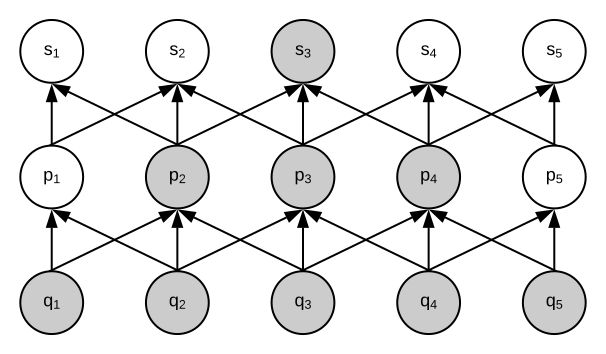
\includegraphics[width=.6\textwidth]{obrazky-figures/receptive.pdf}
    \caption{Receptive field}\label{fig:receptive}
\end{figure}

\subsubsection{Parameter sharing}

A feature of convolution referring to a reuse of of parameter in more than one computation. In matrix multiplication, each weight element is calculated and used only once when computing the output. The weight is multiplied by one element of the input and then never used again. In contrast, convolution keeps it's kernel the same an uses its elements for every output calculation. This brings an advantage of learning just one set of weights for the whole input, rather than computing and remembering a set of weights for each output unit. Parameter sharing has no impact on on forward propagation but it does further improve memory efficiency of a stored model.

\subsubsection{Equivariant representation}

A function is equivariant to another when $f(g(x)) = g(f(x))$. Convolution is naturally equivariant for example to translation\,\cite[p.~339]{deeplearningbook} . Imagine we have an input image and we shift the image some pixels to any direction. When convolution is performed, the same kernel is applied to any set of pixels, therefore the feature the network layer aims to collect can be found in the shifted image as well as in the original. It would just appear shifted in the output feature map. Here we can benefit from parameter sharing in use cases like edge detection. We're interested in the same feature, no matter where it appears on the image. In other use cases, like for example face detection, we might not be interested in the full parameter sharing. Imagine we have a kernel which is trained to detect mouth. In order to work properly, we should restrict this kernel to look for the feature only in bottom portion of the picture, because detecting a mouth on forehead would not result in proper outputs. We'll cover more about multi-kernel convolution layers later.

\subsubsection{Variable size of the input}

Convolution can process data samples of different sizes. When the use case requires to the network to be robust enough to properly process for example images, where each of the sample has different dimensions, this is a problem in matrix multiplication. The network can't apply the fixed size weight matrix on an input of different size. On the other hand, convolution is easy to perform, the situation is really similar to input of a fixed size, just the kernel is applied different amount of times.

\subsection{Pooling}

In neural networks, convolution layer doesn't mean solely convolution is applied. Typically such layer consists of multiple stages:

\begin{enumerate}
    \item \textbf{Convolution stage}: Multiple parallel convolutions are computed which produces a set of linear activations.
    \item \textbf{Detector stage}: Each of the linear activations from previous stage is run through a nonlinear activation function.
    \item \textbf{Pooling stage}: Further modification of the layer.
\end{enumerate}

The last, pooling stage, provides better understanding of the convolution output. Instead of returning a set of features, it reduces redundancy of neighbouring outputs and provides a summary statistics. This helps the network to be invariant small transition of the input. This means that if we translate the input of small amount of pixels, the outputs stay the same. This makes such network more robust. In a situations like a face detection, we don't need to know exact pixel coordinates of a feature, eye for example. We just need to define an are where we're looking for such feature.

There are many pooling operations, let's list some of the most popular ones like \textbf{max pooling}\,\cite{maxpooling} (reports the maximum output in rectangular neighbourhood), average of rectangular neighbourhood, $L^2$ norm of the rectangular neighbourhood, and weighted average of distance from the central pixel.

Invariance of transition is produced by pooling over spatial regions, though pooling layer can learn an invariance to a transformation of other kinds as well. That happens if we pool over outputs of other separately parametrized convolutions. As an example you can see an invariance to slant in cursive on figure\,\ref{fig:pooling}. This principle is accented mainly in maxout networks\,\cite{maxout}.

\begin{figure}[h]
    \centering
    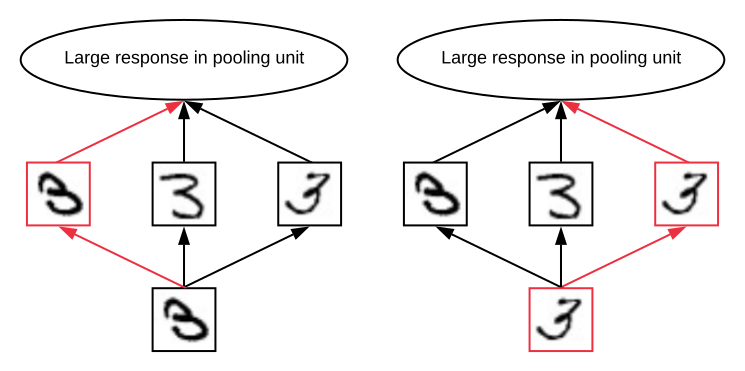
\includegraphics[width=.8\textwidth]{obrazky-figures/pooling.pdf}
    \caption{\textit{Pooling response with learned invariance to slant}: Here we have 3 filters, where all of them had a task to learn a handwritten number 3. Each of them resulted in learning of different slant of the number. When a number 3 is given as the input, one of the filters will match it and cause a high activation in corresponding detector unit. Due to use of pooling, the max pooling unit has a large activation as well, no matter which filter matched the number.}\label{fig:pooling}
\end{figure}

Since pooling can summarise a response of layer over whole neighbourhood of input units, it's not necessary to have the same amount of pooling units as the detector ones. We can leverage pooling to provide downsampling as can be seen in figure\,\ref{fig:downsample}. That further improves performance of the network since it lowers the amount of inputs for the next layer.

\textbf{Pooling with downsampling} is essential step when dealing with input of variable size. Let's say we want to use the convolution to detect a face on images with different resolution. We've learned our detectors to register mouth in the bottom half of the image and another two sets of detectors to locate eyes, each in one of the top quarters. We can use convolution layer with downsampling pooling to provide the required classification. We expect to be provided by 3 activations on the output, and each of the detector has assigned it's portion of the input. It doesn't matter if the portion contains this amount of pixels or much more.

\begin{figure}[h]
    \centering
    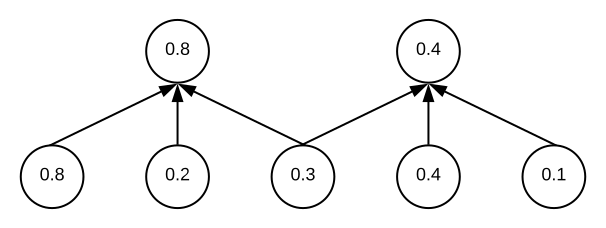
\includegraphics[width=.6\textwidth]{obrazky-figures/downsampling.pdf}
    \caption{Pooling with downsampling}\label{fig:downsample}
\end{figure}

In deep learning this is often the case. We don't refer to convolution as a simple single operation as described in the beginning of this chapter. Such convolution layer with single kernel would be capable of extraction only single feature, although in many spatial locations. Usually many convolutions are applied and performed in parallel. That can provide many different kernels for different features which are interesting for the use case. As a result network can locate many kinds of features at many locations.

\subsection{Strided convolution}

Also when we're already mentioning the downsampling in pooling, this step can be sometimes ommited and simplified even more. Although the result is similar to the pooling with downsample, the logic in based on different assumptions. In pooling we leverage all the information retrieved by the convolutions and simplify the output.

A strided convolution is rather avoiding some of the convolutions at all. That further lowers the computational costs, hence at a risk of not extracting all the features in such detail. In this case we sample pixels in every direction with a step $s$. This $s$ is called a \textbf{stride}. It's also possible to define a separate stride for each step direction.

\begin{figure}
    \centering
    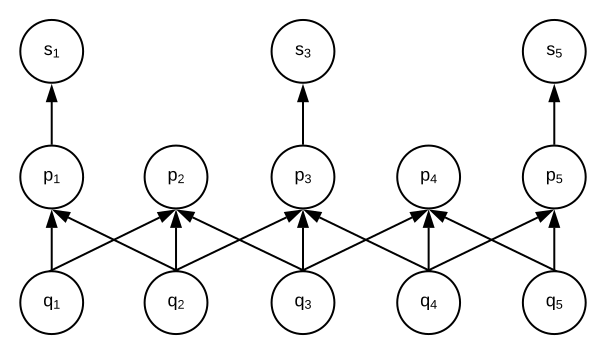
\includegraphics[width=.6\textwidth]{obrazky-figures/conv_down.pdf}
    \caption{Convolution and pooling with downsampling}\label{fig:conv_down}
\end{figure}


\begin{figure}
    \centering
    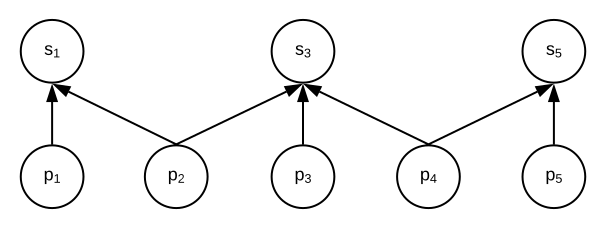
\includegraphics[width=.6\textwidth]{obrazky-figures/strided.pdf}
    \caption{Strided convolution}\label{fig:strided}
\end{figure}

As it can be clearly seen on the images\,\ref{fig:conv_down} and\,\ref{fig:strided} the two step downsampling is computationally more expensive than the strided optimisation.

\subsection{Zero padding}

Another feature which is essential to CNNs implementation is padding with zeros. This maintains the network's ability to preserve the width of its input if needed. The input tensor is padded with zeros on the ends, so a convolution operation doesn't shrink the size of input vector by a fraction of kernel. Without padding we are forced to either keep kernels small, or let the networks shrink in spatial extent. Both are extreme limitations of network's power. Padding allows to control independently both the size of kernel and resolution of the output.

\subsection{Other convolution layer types}

Sometimes our desire is to rather use locally connected layers. This resembles a discrete convolution with small kernel, but without parameter sharing. Therefore this layer type is sometimes called \textbf{unshared convolution}\,\cite{locally_connected}. Unshared type of convolutional layer is useful when we aim to detect features which are local and there's no assumption that the same feature should occur across all the input.

Another type available is \textbf{tiled convolution}\,\cite{tiled_conv} layer. A layer type meant to offer compromise between locally connected layers and convolutional layers. Instead of learning a set of weights for every spatial location, this layer type provides tiling. That means a single set of weights is learned and it is later applied in rotation, providing different set of weighs for neighboring locations. This makes the outcome similar to locally connected layer, while keeping a benefit of lower cost of convolutional layer, since requirements to store parameters would grow by factor of kernel set size, instead of size of whole feature map. A comparison overview of different convolution layer types can be seen on figure\,\ref{fig:compare_layers}

\begin{figure}
    \centering
    \includegraphics[width=.6\textwidth]{obrazky-figures/locally_connected.pdf} \\
    Locally connected \\
    \bigskip
    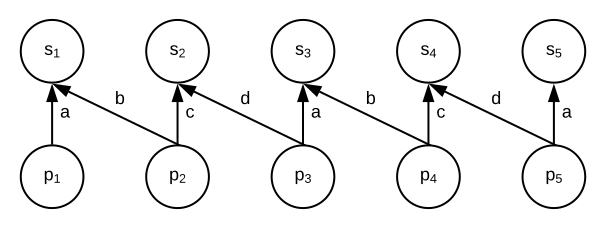
\includegraphics[width=.6\textwidth]{obrazky-figures/convolution_tiled.pdf} \\
    Tiled convolution \\
    \bigskip
    \includegraphics[width=.6\textwidth]{obrazky-figures/convolution_std.pdf} \\
    Standard convolution \\
    \bigskip
    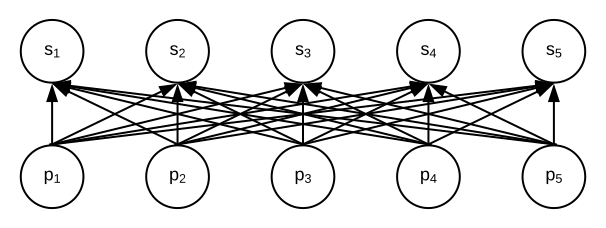
\includegraphics[width=.6\textwidth]{obrazky-figures/fully_connected.pdf} \\
    Fully connected \\
    \bigskip
    \caption{Comparison of convolutional layers}
    \label{fig:compare_layers}
\end{figure}

\section{Capsule neural networks}

Convolutional neural networks are a state-of-the-art of current deep learning. They are hugely popular and they can provide great results and solve problems which were unimaginable before. Despite all their power they embody fundamental drawbacks and limitations\,\cite{capsule_compare}. This and availability of grater computational power lead to creation of Capsule neural networks (CapsNET)\,\cite{capsule}.

\subsection{Rationale}

CNNs operate with features and their recognition. Deeper convolution layer detect
simple features, for example edges or color gradients. Layers higher in the network are designed to detect specific combinations of such features and creates more complex ones. And finally on the very top of the network a dense layer takes the very high level features and provide a prediction of a classification. And since many times the convolution is made invariant to different transformations, this can lead to impossible results. Mere presence of an object provides indication of feature presence. Relation between detected features is not considered at all. When simple features are composed to a more complex one, translational or rotational relationship doesn't play any role.

We've already tackled the way CNN is using to deal with this problem. Pooling and more convolutional layers of smaller kernels are applied to reduce spatial size of information lost during each convolution. This aims to increase the field of view for convolutional layers higher in the network, therefore allows them to locate features in larger portion of the input image. Pooling made CNNs surprisingly effective and top performing architecture so far, though still enhancing loss of information.

Prof. Geoffrey Hinton, one of fathers of deep learning and author of many architectures and algorithms is also the author of capsule neural networks. Hinton wrote\,\footnote{\url{https://www.reddit.com/r/MachineLearning/comments/2lmo0l/ama_geoffrey_hinton/clyj4jv/}}:
\begin{quotation}
    The pooling operation used in convolutional neural networks is a big mistake and the fact that it works so well is a disaster.
\end{quotation}

To demonstrate this drawback imagine a CNN face detector. Deeper layers of network detects parts of facial features. The higher layers combines these parts into complex features like an \textit{eye}, \textit{nose} or \textit{mouth}. Our multi-kernel convolution would allow us to define regions where we expect such features, though we can't define the relation between them. The network can simply recognise an image as a valid face, despite for example the \textit{eye} is rotated to the opposite direction than a \textit{mouth}. A demonstration of such problem can be seen on figure\,\ref{fig:capsule_face}.

\begin{figure}[h]
    \centering
    \includegraphics[height=0.3\textwidth]{obrazky-figures/face_normal.pdf}
    \hspace{10em}
    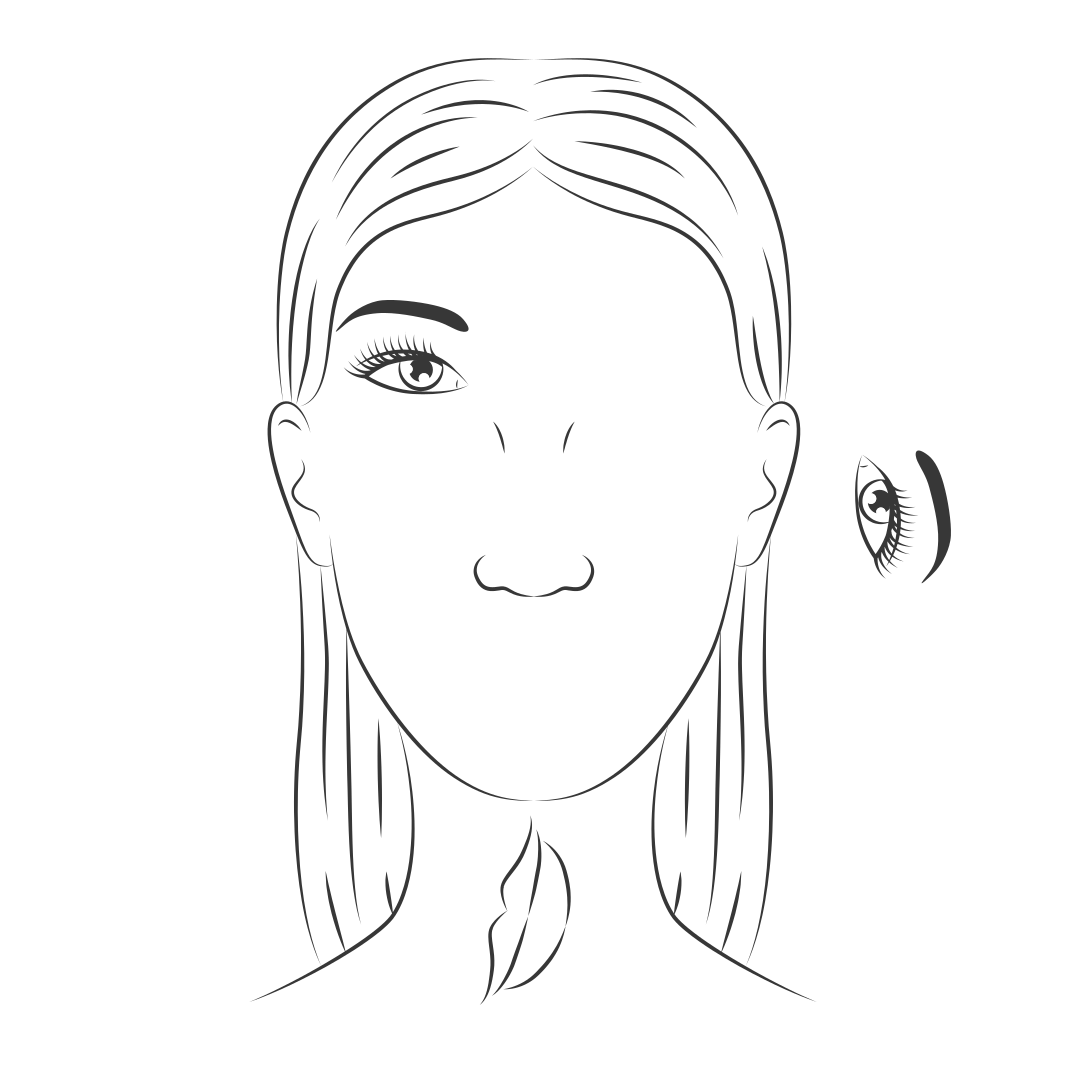
\includegraphics[height=0.3\textwidth]{obrazky-figures/face_disorted.pdf}
    \caption{Both of these images can be evaluated to be a face. Spatial location, relation and pose between simpler features are not considered by this type of network. Both images appear similar to CNN. \textit{Original artwork provided by Freepik\,\cite{freepik}}}
    \label{fig:capsule_face}
\end{figure}

\subsection{Inverse graphics}

Hinton, inspired by computer graphics, tried to explain and reconstruct human brain's visual cognitive functions. The brain itself in fact does the opposite process to \textit{rendering}. Hinton calls it \textbf{inverse graphics}. A visual information is decomposed into a hierarchical representation of objects, which are matched against known, learned patterns. This relationship matrix is stored in our brains. One key factor is that object representation is not dependent on view angle.

So how do we model this hierarchical relationship inside a neural network? Here we can learn from solutions already discovered in another field -- in computer graphics. 3D modeling uses something called a \textbf{pose}. This represents relation between 3D objects and provides a rotation and translation transformation matrix. In neural networks we represent that as a 4D \textit{pose matrix}\,\cite{capsule}. This results in combination of information about object relations with internal representation of object data. Hence it becomes easy for a model to recognise that it just sees a different view of something it already saw before.

\begin{figure}[h]
    \centering
    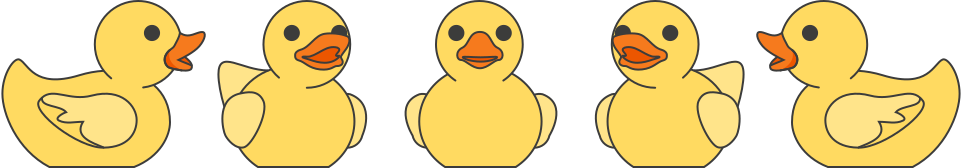
\includegraphics[width=.8\textwidth]{obrazky-figures/duck.pdf}
    \caption{CNN struggles to recognise this is the same object. Human brain, on the other hand, immediately understands that objects on the picture are identical, despite being viewed from multiple different angles. \textit{Original artwork provided by Freepik\,\cite{freepik}}}
    \label{fig:duck}
\end{figure}

Let's discuss situation on the figure\,\ref{fig:duck}. A human looking at this picture can easily recognise, it is a rubber duck viewed from different angles. Our internal representation of rubber duck is independent on the viewing angle. It may be the first time that these particular pictures are shown to you, although you simply know their meaning. Since there's no internal representation of 3D space in CNNs, it really struggles. On the other hand, for CapsNET, this problem is pretty easy since the 3D relations are explicitly modeled. Experiments shown that usage of capsule neural networks can reduce error rate from $20\%$ to $12\%$\,\cite{capsule_compare}.

And this is not the only benefit of usage of capsules. It also significantly lowers the amount of data required to train such network to achieve comparable performance to a CNN. And this make sense, since capsule theory is much closer to the way how brain does work. If a brain tries to learn to distinguish a horse from a cow, it only needs to be presented with few images, at most couple of dozens. CNN would require to be presented by many thousands of image samples, to achieve comparable performance. In this particular aspect we can compare CNNs to a brute-force approach to deep learning.
